\chapter{Asking Wall Street Moguls How They Got Rich}

This lecture has almost no mathematics in the blackboard sense, yet it is quantitative from start to finish. Here the street itself becomes the blackboard: annual revenue, daily trading volume, notional value, planning horizon, and the arithmetic of opportunity are the quantities that organize the argument. The speaker begins with a teaser of access, widens that into a mission on Wall Street, extracts one kind of lesson from Gary Vaynerchuk, a second from a technology executive, and finally a more complete chain from Peter Tuchman outside and then inside the New York Stock Exchange. If we read it carefully, the lecture is not a collection of hustle slogans. It is an inquiry into scale, scarce attention, discipline, asset choice, and the difference between personal wealth and market machinery.

\section{Wall Street as a Search Problem}

The lecture opens with interruption. A man is stopped on the street, the New York Stock Exchange is named, and wealth is immediately tied to a place rather than to a vague abstraction. This matters. We are told, before any extended explanation, that the route to money will be investigated where money is moved, traded, and defended.

The narrator then steps back and states the larger premise. The New York Stock Exchange is presented not merely as a famous building but as a concentration of global financial activity. Trillions of dollars are said to move through its doors each day, and the day's objective is made explicit: learn from rich operators and somehow gain access to the exchange itself. In that sense, the lecture is structured as a search problem. Knowledge is local, gated, and embodied in people who are difficult to stop.

To keep the scales straight, it is helpful to collect the principal quoted magnitudes at the outset.

\begin{table}[h]
\centering
\begin{tabular}{|l|l|l|}
\hline
Quantity & Symbol & Reported scale \\
\hline
VaynerX annual revenue & $R_{\mathrm{VaynerX}}$ & about $3.4\times 10^8\ \mathrm{USD/yr}$ \\
Single-trader daily volume & $V_{\mathrm{trader}}$ & about $5\times 10^8$ to $10^9\ \mathrm{USD/day}$ \\
Floor share volume & $Q_{\mathrm{floor}}$ & about $1.2\times 10^9\ \mathrm{shares/day}$ \\
Floor notional value & $V_{\mathrm{floor}}$ & about $10^{12}\ \mathrm{USD/day}$ \\
Listed companies & $n_{\mathrm{listed}}$ & more than $3\times 10^3$ \\
Usable tech horizon & $H_{\mathrm{forecast}}$ & about $12$ to $18$ months \\
\hline
\end{tabular}
\caption{Quoted scales that anchor the lecture.}
\end{table}

What is pedagogically important is that these scales arrive before formal explanation. The lecture wants us to feel magnitude first, then ask how such magnitude is produced.

\section{Gary Vee: Scale and the Hidden Operating Layer}

The first sustained stop is Gary Vaynerchuk. The sequence is deliberate. We are first given identity, then money, then operating structure. Gary says that he made his millions in marketing, but the lecture does not leave the matter there. It quickly pushes toward scale.

If we write $R_{\mathrm{VaynerX}}$ for the annual revenue of the main operating company named in the interview, then the quoted magnitude is
\begin{equation}
R_{\mathrm{VaynerX}} \approx 3.4\times 10^8\ \mathrm{USD/yr}.
\end{equation}
Alongside that, the speaker places Gary's personal income in the range of hefty or high eight figures. The exact number is not fixed, but the scale is the point. The lecture is careful to frame authority not as internet fame alone, but as the authority of someone running a large business day to day.

Gary then resists the simplified image of himself as a motivational speaker or content personality. He insists that he is operational, even saying that internally he is as much COO as CEO. This is the decisive pivot. The lecture moves from money as outcome to management as mechanism.

The core claim is that the most important activity of a chief executive is often not taught in business school: one must scale what appears unscalable, especially with the human beings who most affect the outcome. He gives a concrete example. Even under severe time pressure, he will spend an hour and a half at dinner with a small group of teammates simply to know what they care about: title, money, work-life balance, and the rest. The argument is not sentimental. It is organizational.

\subsection{Question \& Answer}

\paragraph{Question.} Why should ``non-scalable'' human interactions become more valuable precisely when AI and technology make everything else scale more easily?

\paragraph{Answer.} The lecture's answer is economic rather than mystical. When routine coordination, content generation, and distribution become cheaper, the scarce complement is no longer mere throughput. It is trusted human attention from the principal to the few people who matter most. Gary's dinners, check-ins, and one-on-one conversations are therefore not failures of scale. They are scarce interventions inside a scalable machine. The claim is that cheap automation increases the marginal value of costly, credible, personal attention.

The lecture does not turn this into a formal theorem, and we should not force one. But the logical structure is clear: abundance in one layer creates scarcity in another.

\section{Attention, Distribution, and Urgency}

Having established Gary's operating scale, the lecture widens from internal management to market-facing leverage. Here the key word is attention. Gary argues that organic social media creative is still radically undervalued, grossly misunderstood, and capable of changing a business when a single post reaches a sufficiently large audience. The example is framed almost as disbelief: can one post reach ten million and begin changing everything? His answer is yes.

What matters in the lecture is not the sociology of social platforms but the economic form of the claim. Distribution is treated as underpriced leverage. If a person or company learns to capture attention organically, then the market can move before traditional institutions have even recognized what is happening. This is why the lecture immediately turns from content to education. The complaint is that institutions still teach old communication forms while underestimating the actual attention market now in front of us.

That logic then sharpens into a harder claim about debt. For a person who is entrepreneurial or creatively inclined, debt-financed college can be irrational if it delays entry into the market where attention is acquired and converted. Again, the lecture does not give us a formal discounted-cash-flow argument, but the sequencing is unmistakable: first underpriced distribution, then mispriced education, then the cost of delay.

The lecture's final move in this section is existential. If attention is the currency that matters, then hesitation is not merely inefficient; it is life-denying. The question of mortality is used to compress time. The audience is told to tune out parents, admired figures, and peers, because one has exactly one life to live. This is not mathematics, but it functions like boundary data. The time horizon of life itself is introduced as the outer constraint on all local optimization.

\section{Recap, Sponsor Interlude, and the Return to the Street}

After Gary, the narrator performs an important pedagogical move: he restates the lesson in simpler language. Attention is everything. Organic content remains the strongest marketing instrument. If nobody has your audience's attention, then there is no real business to speak of. This recap matters because the lecture wants synthesis, not merely quotation.

The lecture then pauses for a sponsor read. Even this interruption is not structurally random. The sponsor segment effectively says that the lesson about attention can itself be operationalized: content can be clipped, distributed, captioned, and scheduled at scale. In other words, the interlude mirrors the previous argument. We should preserve that fact, even if we compress the segment later.

Only then do we return to the street. The return is not smooth. The narrator repeatedly fails to stop passersby. People are heading to meetings, refusing interviews, or simply moving too quickly. This friction is not filler. It keeps alive the governing fact of the lecture: access to rich knowledge is costly, contingent, and sometimes humiliatingly hard.

A small but concrete constraint is introduced here. One passerby suggests that the closing bell occurs at four o'clock and that brokers may flow out between four and four-thirty. This is a useful reminder that access is not only social but temporal. Timing enters the lecture as a practical variable.

\section{Discipline, Stoicism, and Cash-Flow Heuristics}

The next street-level broker encounter is rougher and less polished. Some of the advice is clearly personal bias and should remain marked as such. But the lecture does extract a usable mechanism from the conversation: discipline. The broker traces his discipline to the United States Marine Corps and then folds that into a stoic vocabulary. Everything is fleeting. One must judge oneself first, answer to oneself and God, and treat fame, fortune, and even the present video as temporary.

We should not over-formalize this. The operative point is that the lecture temporarily moves from revenue and attention to self-command. That movement matters because it prepares us for the more structured corporate-finance language that follows.

The Snowflake executive then shifts the register again. He identifies himself as a chief revenue officer, places his own wealth in technology, and gives the lecture a short public-market primer. He advises firms to stay private until they have a defined market and a defined go-to-market plan; only then, when additional funding is needed for execution, should public capital enter the story.

A second timing heuristic appears here. Asked about the future of technology, he refuses the comfort of a long-range forecast and compresses the usable decision horizon:
\begin{equation}
H_{\mathrm{forecast}} \in [12,18]\ \mathrm{months}.
\end{equation}
That is, five years is too far and too unstable; a year to a year and a half is the interval in which serious operational decisions can still be made responsibly. This is an important note-writing point, because it tells us how the lecture thinks about uncertainty. Long narrative forecasts are cheap; short operational forecasts are costly and actionable.

\subsection{Question \& Answer}

\paragraph{Question.} What does the line ``cash flow is king before profitability'' mean in the limited sense of this lecture?

\paragraph{Answer.} The interviewee is not stating a formal accounting identity. He is stating a survival principle. Before a business reaches durable profitability, it must continue to finance its own operation long enough to keep executing. Cash flow therefore has priority because it determines whether the firm remains alive while strategy matures. Only after that does profitability, and later public-market valuation, fully enter the picture.

The speaker then adds another tension. He says people should save everything they can, yet also agrees that one cannot save one's way to wealth. That distinction is worth preserving. Saving is treated as a path to security; wealth requires ownership, scale, or leverage beyond the wage relation. This is consistent with the later ``stocks, not stuff'' theme.

\section{Peter Tuchman: Stocks, Not Stuff}

The lecture's richest single interview begins with Peter Tuchman. Here the argument becomes more coherent and cumulative. Tuchman first addresses the younger generation not as a moral scold but as a consumer class. His claim is that the crucial financial shift is from buying stuff to buying stocks.

The mechanism is simple and should be kept simple. Most discretionary consumer purchases are said to lose value immediately after purchase. Stocks, by contrast, are claims on enterprises that may rise in value over time. This is not a guarantee, and the lecture does not pretend otherwise. But it is a clean asymmetry: consumption satisfies the present urge; ownership gives one a stake in future productive activity.

\subsection{Question \& Answer}

\paragraph{Question.} Why ``stocks, not stuff''?

\paragraph{Answer.} Because the lecture wants to separate two different arithmetics. Stuff is generally purchased for immediate use or desire, and its resale value usually falls at once. Stocks are risky, but they are ownership claims rather than consumption events. The point is not that every stock appreciates. The point is that consumption and ownership obey different financial logics, and younger people often blur them.

Tuchman then gives the lecture its strongest adversity story. He says he was virtually penniless, that he spent an extended period not making money, and that for a time he hid under the covers. But the lecture does not allow the story to settle there. He has a wife and children, so hiding is not an equilibrium. He begins to dress up, show up, and go to work each day even while earning nothing. He keeps visible.

This is one of the few places in the lecture where a causal structure is explicit enough to diagram.

\begin{figure}[h]
\centering
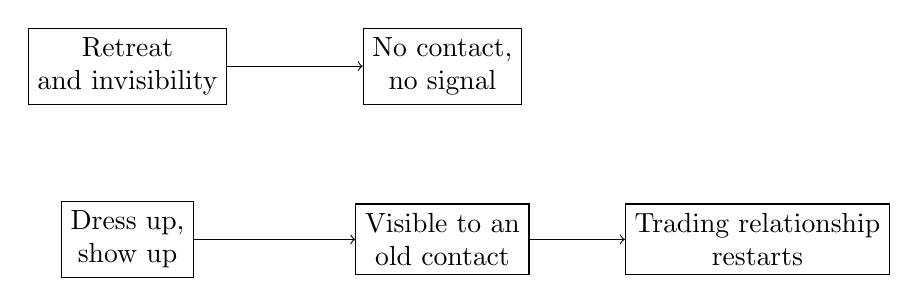
\begin{tikzpicture}[x=1cm,y=1cm]
\node[draw, rectangle, align=center] (a) at (0,0) {Retreat\\and invisibility};
\node[draw, rectangle, align=center] (b) at (4,0) {No contact,\\no signal};
\node[draw, rectangle, align=center] (c) at (0,-2.2) {Dress up,\\show up};
\node[draw, rectangle, align=center] (d) at (4,-2.2) {Visible to an\\old contact};
\node[draw, rectangle, align=center] (e) at (8,-2.2) {Trading relationship\\restarts};
\draw[->] (a) -- (b);
\draw[->] (c) -- (d);
\draw[->] (d) -- (e);
\end{tikzpicture}
\caption{A schematic of Tuchman's verbal mechanism. Opportunity is not treated as magic; it is treated as something whose probability rises when one remains visible.}
\end{figure}

The story resolves when an old Wall Street contact sees him on the subway, asks how he is doing, hears the truth, and restarts a trading relationship. The lecture's conclusion is not that luck is unimportant. It is that luck needs a surface on which to land. Hiding removes that surface.

\section{Inside the New York Stock Exchange}

At the moment Tuchman agrees to take the narrator inside, the lecture changes register. We move from biography and principle to mechanism and scale. The New York Stock Exchange is no longer only symbolic. It becomes a machine whose arithmetic can be sketched.

We begin with the simplest object.

\begin{definition}
For a trade of $q$ shares at price $p$ dollars per share, the notional dollar value of the trade is
\begin{equation}
N = q\,p.
\end{equation}
\end{definition}

Tuchman illustrates this with an example close enough to turn into a worked calculation. For $1000$ shares of a stock priced around \$400 to \$500, the notional value is already in the hundreds of thousands of dollars:
\begin{align}
N_{\min} &= 1000 \times 400 = 4\times 10^5\ \mathrm{USD},\\
N_{\max} &= 1000 \times 500 = 5\times 10^5\ \mathrm{USD}.
\end{align}
So even a trade that sounds modest in share count can imply
\begin{equation}
N \in [4\times 10^5,\,5\times 10^5]\ \mathrm{USD}.
\end{equation}

The lecture then adds a second quantitative comparison. Tuchman says that his own desk may trade on the order of half a billion to a billion dollars per day, but that the floor itself may handle nearly a trillion dollars of notional value. If we write those as
\begin{align}
V_{\mathrm{trader}} &\in [5\times 10^8,\,10^9]\ \mathrm{USD/day},\\
V_{\mathrm{floor}} &\approx 10^{12}\ \mathrm{USD/day},
\end{align}
then the scale comparison becomes
\begin{equation}
\frac{V_{\mathrm{trader}}}{V_{\mathrm{floor}}}\sim \frac{10^9}{10^{12}} = 10^{-3}.
\end{equation}
This is a very useful calculation. It explains how a billion dollars can be both enormous in ordinary life and modest relative to the aggregate machine of the exchange floor.

The lecture also gives a share-volume number and a listed-company count:
\begin{align}
Q_{\mathrm{floor}} &\approx 1.2\times 10^9\ \mathrm{shares/day},\\
n_{\mathrm{listed}} &\gtrsim 3\times 10^3.
\end{align}
Again, we should not over-interpret the precision. The interview is not a market microstructure seminar. But these quantities are enough to tell us what kind of object the NYSE floor is: a coordination device operating at extraordinary scale.

A final numerical comparison appears when Tuchman contrasts the pre-technology floor with the present one. He says that now he can send out roughly $1000$ orders in five to ten seconds. That translates into an implied rate of
\begin{equation}
\text{order rate} \approx \frac{1000}{5\text{ to }10\ \mathrm{s}} \approx 100\text{ to }200\ \mathrm{orders/s}.
\end{equation}
The exact rate is only illustrative, but the point is sharp. Technology has compressed execution time so drastically that the old paper-based exchange and the modern exchange are separated not merely by convenience but by order-of-magnitude differences in throughput.

\subsection{Question \& Answer}

\paragraph{Question.} How can someone say that he trades a billion dollars a day and then immediately suggest that this is ``not that much''?

\paragraph{Answer.} Because the unit of comparison has changed. Against household wealth, firm budgets, or even most businesses, a billion dollars per day is overwhelming. Against a trading floor handling activity on the order of a trillion dollars per day, it is roughly one-thousandth of the whole. The lecture's lesson is that scale is relational. The same number changes meaning when the ambient machine changes size.

The section closes with the exchange bell and its ceremonial history. Since 1903, the opening and closing bells have marked participation in a highly exclusive public ritual involving heads of state, CEOs, IPOs, charities, and other symbolic figures. This matters because the lecture has now fully joined two things that were separate at the beginning: the theater of Wall Street and its quantitative machinery.

\section{Summary}

The lecture leaves us with a coherent cluster of claims. First, wealth is not presented as a mysterious personal trait; it is tied to systems, institutions, and concrete magnitudes. Second, in a world of automation and AI, non-scalable human attention can become more valuable rather than less. Third, public claims about finance must be read at the right level: revenue, cash flow, notional value, and market scale are not interchangeable. Fourth, the lecture sharply separates consumption from ownership, and security from wealth. Finally, the street-level moral at the end is narrower than many motivational lectures allow: money does not buy happiness, but it does buy freedom, and freedom changes the geometry of a life.